\section{sEMG Classification}

In order to justify the need for deep sEMG classifiers, it is important to briefly discuss why shallow classifiers are inappropriate. Shallow classifiers (and really all of classical machine learning) relies on \emph{feature engineering}, or the creation of robust features which represent the data in a precise manner \cite{bddl}. This is very powerful, but it also comes with the assumption that the same fundamental process is generating all data points, that is the same feature set that works at time $a$ for person $x$ works at time $b$ for person $y$. However, in the case of surface electromyography, all brains and bodies are completely unique, which means that a classical, engineered feature set is neither robust between subjects or between repetitions (over time) \cite{dlot}. Therefore, we must turn to deep learning, to \emph{learn features from the data}, which are more robust over time and over subjects.

\subsection{Deep Learning}

Much of the previous work in sEMG classification (and time series classification in general \cite{dltsr}) with deep learning revolves around convolutional neural networks. In this subsection, notable and influential recent work will be highlighted. \cite{atz_cnn} very clearly demonstrated the power of convolutional neural networks with respect to sEMG classification, namely their flexibility and ease of use (due to feature learning vs feature engineering). This work is expanded in \cite{primary}, in which the authors use convolutional neural networks, wavelet transformations, and deep transfer learning to slightly improve on the results highlighted in \cite{atz_cnn}. \par
This study instead explores a new direction for both time series classification in general and for sEMG classification in particular: attention. In the last few years of language modeling, attentional models have proven more and more utilitarian, managing to solve problems of long term memory (which are commonplace in time series and language) while also managing to avoid the training and gradient issues of recurrent neural networks. Attention is a flexible, intuitive mechanism with lots of untapped application. In this study, the simple, feed-forward model of attention  described in \cite{raffel2015feedforward} is expanded upon. The attention mechanism is shown in \autoref{fig:okokt}. 


\begin{figure}[h]
\caption{%
A simple model of temporal attention.
}
\label{fig:okokt}
\begin{center}
\includegraphics[scale=0.75]{att}
\end{center}
\end{figure}

The mechanism works as follows: First time series data, an $(M,N)$ matrix (where $M$ represents timesteps and $N$ represents features or channels). This matrix is transposed into an $N$ by $M$ matrix. In this matrix, an observation at a single row represents all timesteps of that feature or channel. For example, row $x$ represents the time series produced by the feature $N = x$. This matrix is then fed in row by row to a standard, feedforward layer, using the softmax activation function. Thus, for each timestep of each feature, an importance (referred to as an "attention score") is calculated. Next, these are summed across time, producing a single number per feature, which represents the overall importance of the feature within that sample. As per \cite{raffel2015feedforward}, this simple mechanism, akin to a parametric time weighted average, actually successfully solves long term memory problems where order is not very important (or in this case, where memorization is to be avoided).


%\begin{figure}[h]
%\caption{%
%A motor unit, consisting of: \emph{1} an Axon, \emph{2} a junction site, \emph{3} a Myocyte, and \emph{4} Myofibrils. The Axon sends electrical signal through the junction cite, causing the all of the myofibrils (and thus the entire myocyte) to contract.
%}
%\begin{center}
%\label{fig:okok}
%\fbox{\includepdf[height=5cm]{fig/att}}
%\end{center}
%\end{figure}
%
%
